\section{Borders Filter}

Edges are widely used in computer vision, they contain rich information about texture 
and geometry, for this reason edges are features that are usefull for several tasks, 
such as object recognition, object traking, etc.


The Sobel filter is a wellknown edge detector. To apply this filter is necessary to 
convolve the image with two 3x3 matrix, to find intensity changes in vertical and 
horizontal directions:

\begin{center}

\includegraphics[scale=0.35]{images/sobel}
\end{center}

Then both results are merged using the bellow expression and then a threshold is used to filter out non interest areas:

\begin{equation}
G = \sqrt{G_x^2+ G_y^2}
\label{eq:sobelGrad}
\end{equation}

This filter is applied directly into a grayscale representation of the original RGB image. Obtaining a binary image 
that contains edges representing geometrical and visual changes in the scene.

%edges image

This image can be used along with the depth map to reduce the point cloud size. Rejecting all 3D points not corresponding
to this edges. We are interested in find correspondences between the two clouds, for this reason, edge filtering was applied
to the image instead of the depthmap. Because using this approach it is possible to find corresponcendes between rich textured 
surfaces, even if they don't exhibit local geometrical changes.

The applied threshold was low, in order to have thicker edges. Because if too few points pass the filter, important information 
could be lost, difficulting a correct alieation. 


In combination with a low threshold, more points where added, based on their 
distance to the sensor:

\begin{equation}
\bar{z} = \frac{1}{8} \sum \limits_{p \in neighboor} p.z
\end{equation}

The neighborhood is defined as shown in figure ~\ref{fig:neighboor}. Then points satisfying the following condition where added:

\begin{equation}
p.z <= \bar{z}
\end{equation}

This filter is applied to both, source and target captures. Making this, it is possible to apply a very useful filtering: remove 
from the edges binary image all the points that are not simultaneously in both captures. For this, the rotation and translation 
of the source 2D image that minimizes the distance to the target 2D image is applied and then an AND operation is applied between 
the two images. As result, we work with two point clouds that have a huge amount of overlaping points, improving the alineation 
result.


A Sobel filter was used to obtain a representative set of points, avoiding that walls and another 
plain surfaces containing a huge amount of data, lead to an incorrect alineation.

\begin{figure}[h!]
\begin{center}
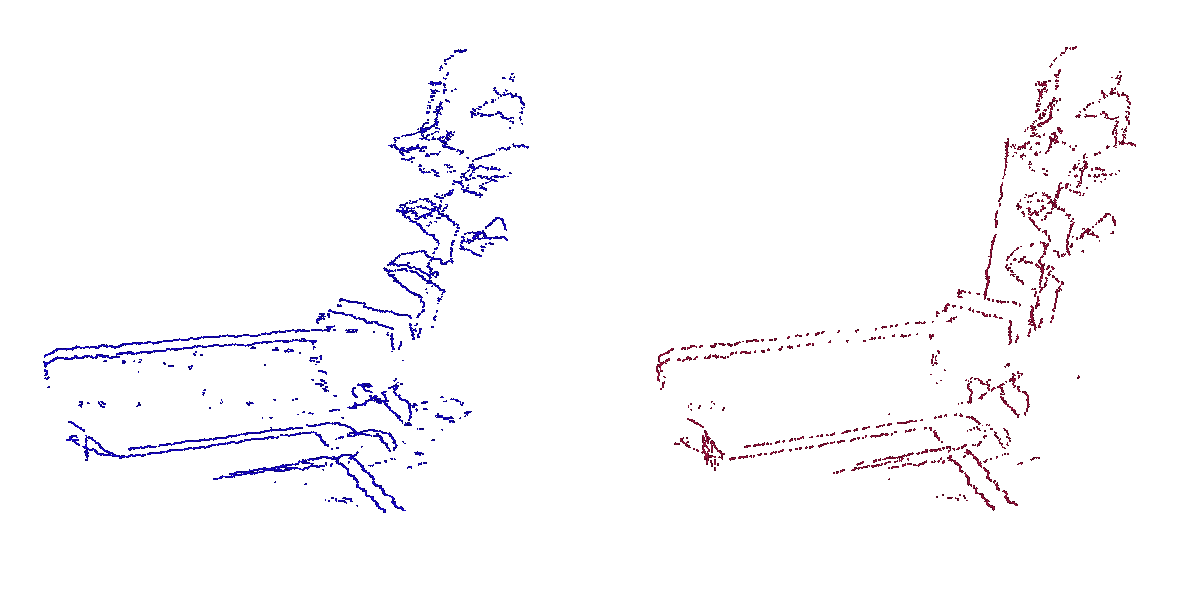
\includegraphics[scale=0.35]{images/sobel_v_h.png}
\caption{Left: Sobel vertical filtered point cloud, Right: Sobel horizontal filtered point cloud}
\end{center}

\begin{center}
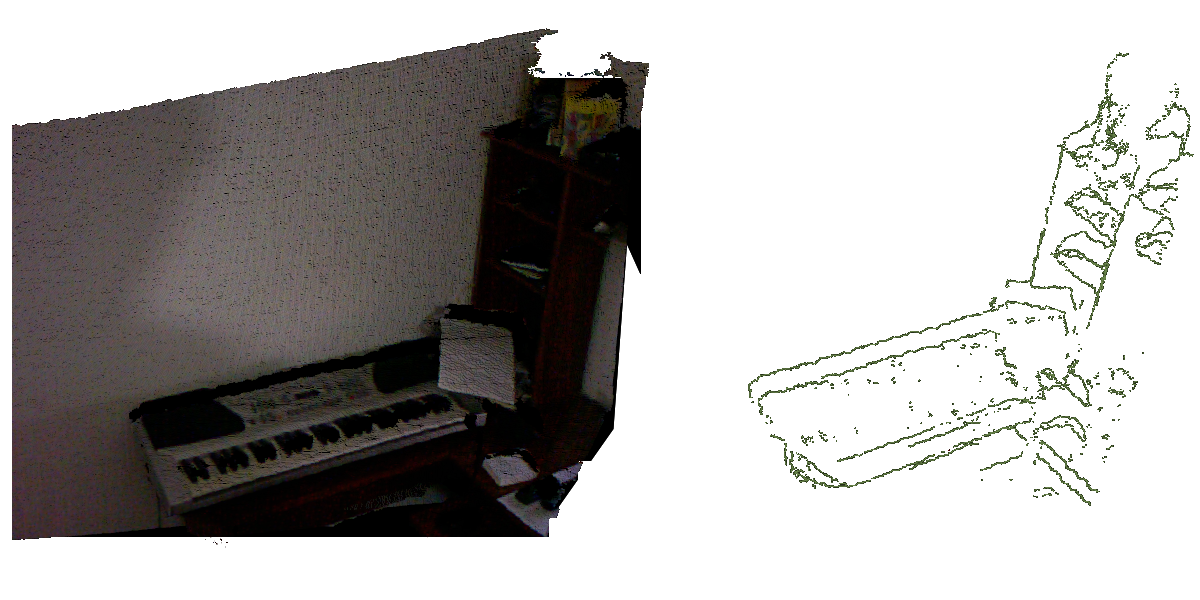
\includegraphics[scale=0.35]{images/sobel_o_g.png}
\caption{Left: Original point cloud, Right: Sobel filtered point cloud}
\end{center}
\end{figure}

There are more advanced edge filtering techniques, such as the Canny edge filter, but it involve 
a larger set of convolutions and operations. We dont need an high accuracy edge detection, the Sobel 
filter is enough to reduce the set of points used in the alineation process.

